\begin{frame}{Langevin dynamics}
	\vspace{-12pt}
		\tikzstyle{every picture}+=[remember picture]
		\tikzstyle{na} = [baseline=-.5ex]
		\begin{equation*}
			\ddot{x} =  
			\tikz[baseline]{\node[fill=blue!20,anchor=base] (t1){$F$};} 
			-
			\tikz[baseline]{\node[fill=red!20,anchor=base] (t2){$\nabla U$};}
			-
			\tikz[baseline]{\node[fill=green!20,anchor=base] (t3){$\gamma \dot{x}$};}
			+
			\tikz[baseline]{\node[fill=orange!20,anchor=base] (t4){$\sqrt{2T\gamma}\xi_t$};}
		\end{equation*}
	\begin{tabular}{l l}
	\begin{minipage}{.85\textwidth}
		\begin{itemize}
			\item constant force $ F $ \tikz[na]\node [coordinate] (n1) {}; 
			\item force caused by periodic potential  \tikz[na]\node [coordinate] (n2) {};$U$
			\item friction, proportional to the velocity \tikz[na]\node [coordinate] (n3) {};
			\item Brownian motion \tikz[na]\node [coordinate] (n4) {};
		\end{itemize}
		\begin{tikzpicture}[overlay]
			\path[->]<1-> (n1) edge [bend right] (t1);
			\path[->]<1-> (n2) edge [out= 95, in=-70] (t2);
			\path[->]<1-> (n3) edge [out=0, in=-30] (t3);
			\path[->]<1-> (n4) edge [out=-20, in=-50] (t4);
		\end{tikzpicture}
	\end{minipage}
	\begin{minipage}{0.16\textwidth}
		\flushleft
		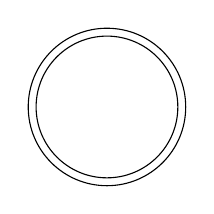
\begin{tikzpicture}
			\draw (0,0) circle (1cm)
						circle (.9cm);
		\end{tikzpicture}
	\end{minipage}
	\end{tabular}
	\begin{tabular}{l l}
		\begin{minipage}{0.5\textwidth}
			\vspace{-1.9cm}
			\begin{block}{Underdamped}
				Particle needs infinite time to reach its final velocity
			\end{block}
		\end{minipage}
		&
		\begin{minipage}{0.5\textwidth}
			\vspace{-.3cm}
			\begin{block}{Overdamped}
				Very high friction\\
				$ \rightarrow $ particle instantaneously reaches its final velocity $ v_f $
				\vspace{-5pt}
				\begin{equation*}
				\gamma v_f = F - \nabla U + \sqrt{2T\gamma}\xi_t
				\end{equation*}
			\end{block}
		\end{minipage}
	\end{tabular}
\end{frame}



